\section{Antecedentes y justificación}
Esta sección se centra en describir el ecosistema actual del desarrollo e investigación 
de modelos de inteligencia artificial y justificar la necesidad de la creación de un
estándar dentro de un equipo. Se presentan datos e información general sobre las 
tecnologías más relevantes utilizadas en el proyecto, dando una visión general 
de por qué se eligieron, teniendo en cuenta las últimas tendencias que están
surgiendo en el ámbito del aprendizaje automático.

\subsection{Justificación}
Cada año, más empresas y organizaciones invierten recursos significativos en 
proyectos de IA. Como se muestra en la figura \ref{fig:ai-investement},
en 2021 la inversión global superó los 270 mill millones de dólares \cite{Letzing2024-nn},
lo que supone un aumento del 40\% de la inversión con respecto al año anterior.
Este crecimiento de la inversión busca aprovechar al máximo el potencial de la IA 
y sacar provecho de su ventaja competitiva. Un ejemplo notable de este fenómeno es OpenAI, 
una empresa que ha sido valorada en más de 80 mil millones de dólares \cite{noauthor_2024-uj} con el record de crecimiento 
en el numero de usuarios más rápido de la historia \cite{Armenta2023-xt}. Todo esto
gracias a su modelo de lenguaje GPT-3, que ha demostrado cómo una aplicación de 
inteligencia artificial puede impactar significativamente en la vida de las personas.

\begin{figure}[ht]
    \centering
    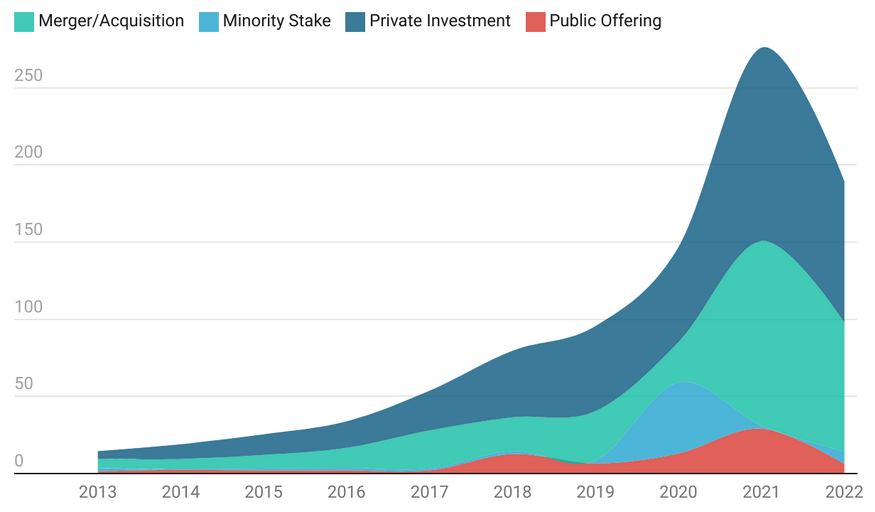
\includegraphics[width=\textwidth]{ai-investement.png}
    \caption{Inversión global en IA en miles de millones \cite{Letzing2024-nn}.}
    \label{fig:ai-investement}
\end{figure}

Nos encontramos en un momento en el que la demanda de equipos cualificados 
que puedan hacer frente a los nuevos desafíos es mayor que nunca. La complejidad
de los proyectos de IA también está en aumento, ya que las aplicaciones de IA
se vuelven más sofisticadas, abarcan una gama más amplia de funciones, requieren
un mayor número de datos y los modelos se vuelven cada vez más complejos. Esta
situación a forzado a las empresas a buscar nuevas formas de gestionar sus proyectos
que han llevado a la creación de nuevas metodologías, adaptadas a las necesidades
a los nuevos retos que se presentan. Si bien es cierto que mucha información es
compartida con la comunidad, existe un gran secretismo en torno a la forma de operar
de las empresas más grandes, lo que dificulta la adopción de estas metodologías.
Podemos resaltar positivamente el caso de Meta \cite{metaia}, que es el mayor 
referente en cuanto contribución y apertura de sus desarrollos en IA.\medskip

Por todo ello, es necesario realizar contribuciones que se centren en el como 
se debería operar dentro de un equipo. Se requiere de una referencia clara sobre las 
directrices que se deben aplicar para poder implementar un estándar tecnológico y
operacional dentro de un grupo de trabajo, así como las herramientas, metodologías y buenas prácticas
a seguir para hacer un uso eficiente de los recursos y obtener resultados de calidad.
Este documento representa un estándar que se ha aplicado en base a unas necesidades
concretas y, aunque no está pensado para poder ser adoptado de forma literal por otros equipos,
se muestra el camino que se ha seguido desde la adopción de plataformas MLOps hasta la creación
de un sistema de conocimiento para la reutilización de trabajo. La justificación de este
documento es exponer el trabajo realizado y servir como referencia equipos que quieran implementar
un estándar similar o busquen inspiración para crear el suyo propio.

\subsection{Estado del arte}
La sección de estado del arte se centra en recopilar información sobre las tendencias
actuales dentro del ámbito del aprendizaje automático y la inteligencia artificial.
Debido a la diversidad de ramas que abarca la creación de un estándar tecnológico y
operacional, se han seleccionado aquellas que se consideran más relevantes o presentan
un mayor peso en cuanto a la toma de decisiones.

\subsubsection{Diseño Atómico}
El diseño atómico es una metodología de diseño que se centra en la creación
de sistemas modulares y reutilizables. La idea principal es dividir
las diferentes funcionalidades de un sistemas en sus partes más fundamentales,
de manera que cada una de estas partes pueda ser reutilizada en diferentes
contextos. Este enfoque permite tener un mayor control sobre cada una de las
partes del sistema, facilitando su mantenimiento, documentación y reutilización.
Originalmente, el diseño atómico ha sido aplicado en el diseño de interfaces
de usuario, pero su filosofía puede ser aplicada a cualquier sistema de diseño
modular. En el contexto de este proyecto, el diseño atómico se aplicará al
diseño de un sistema de componentes para el desarrollo de modelos de aprendizaje
automático.\medskip

Dentro del diseño atómico, los componentes se dividen en cinco categorías
principales, que representan diferentes niveles de abstracción. Estas categorías
son: átomos, moléculas, organismos, plantillas y páginas. Cada una de estas
categorías representa un nivel de abstracción diferente, y se relaciona con
las demás categorías de manera jerárquica. La figura \ref{fig:atomic-design}
muestra la estructura tradicional del diseño atómico. 

\begin{figure}[ht]
    \centering
    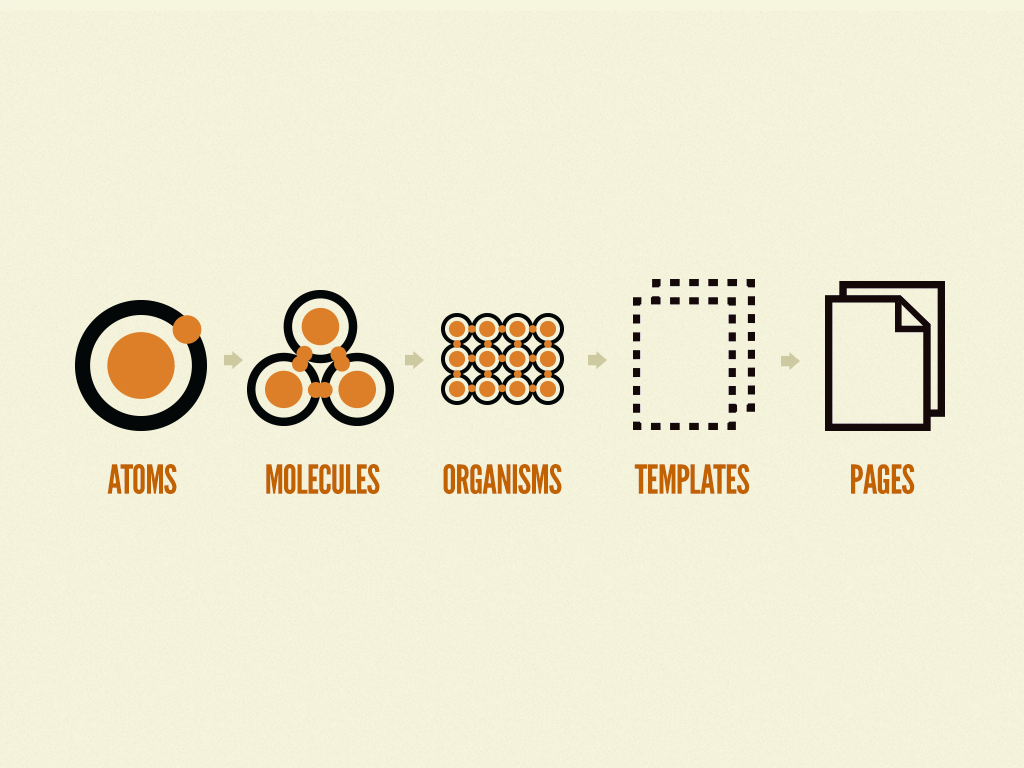
\includegraphics[width=0.7\textwidth]{atomic-design-process.png}
    \caption{Estructura tradicional diseño atómico.}\label{fig:atomic-design}
\end{figure}

A continuación, se describen brevemente cada una de las categorías:
\begin{itemize}
    \item \textbf{Átomos:} Los átomos son los componentes más básicos de un sistema
    de diseño. Representan las funcionalidades más fundamentales, solo tienen
    una responsabilidad y no dependen de otros componentes.
    \item \textbf{Moléculas:} Las moléculas son la combinación de varios átomos
    para formar una funcionalidad más compleja. Representan la combinación de
    diferentes funcionalidades básicas para formar una funcionalidad más compleja.
    \item \textbf{Organismos:} Los organismos son la combinación de varias moléculas
    y átomos para formar una funcionalidad completa.
    \item \textbf{Plantillas:} Las plantillas son la combinación de varios Organismos
    para dar forma a un contenido.
    \item \textbf{Páginas:} Las páginas son la combinación de varias plantillas.
\end{itemize}

Esta estructura jerárquica permite que los componentes sean reutilizados en
diferentes contextos, y que cada uno de ellos pueda ser modificado de manera
independiente. Además, se facilita la documentación y el mantenimiento de los
componentes, ya que cada uno de ellos es independiente de los demás. Podemos
ver multitud de ejemplos de diseño atómico en grandes empresas y que nosotros utilizamos
a diario, como por ejemplo en la creación de sistemas de diseño Microsoft Fluent
Design o Google Material Design entre otros.\medskip

Aunque el diseño atómico se ha aplicado tradicionalmente a la creación de interfaces
de usuario, su filosofía puede ser aplicada a cualquier sistema de diseño modular.
En el contexto de este proyecto, el diseño atómico se aplicará para la creación de un
sistema de componentes en el desarrollo de modelos de aprendizaje automático.
Traeremos la filosofía del diseño atómico y la adaptaremos a nuestro contexto,
con las particularidades y necesidades que requiere el desarrollo de modelos de
aprendizaje automático. 

\subsubsection{Machine Learning Operations (MLOps)}
El desarrollo de modelos de aprendizaje automático es un proceso complejo que implica
la recopilación de datos, la creación de modelos, la evaluación de los modelos y su
puesta en producción. Cada una de estas etapas requiere de diferentes herramientas y
prácticas, y es importante que estas herramientas y prácticas estén integradas de manera
coherente para garantizar la eficacia del proceso. Los principios de MLOPs son una serie de prácticas y herramientas que se utilizan
para gestionar el ciclo de vida de los modelos de aprendizaje automático. Como se muestra en la
figura \ref{fig:mlops-workflow}, este enfoque busca aplicar las mejores tendencias dentro de la 
ingeniería de software al desarrollo de modelos, con el objetivo de mejorar la eficiencia, la 
calidad y la escalabilidad.\medskip

\begin{figure}[ht]
    \centering
    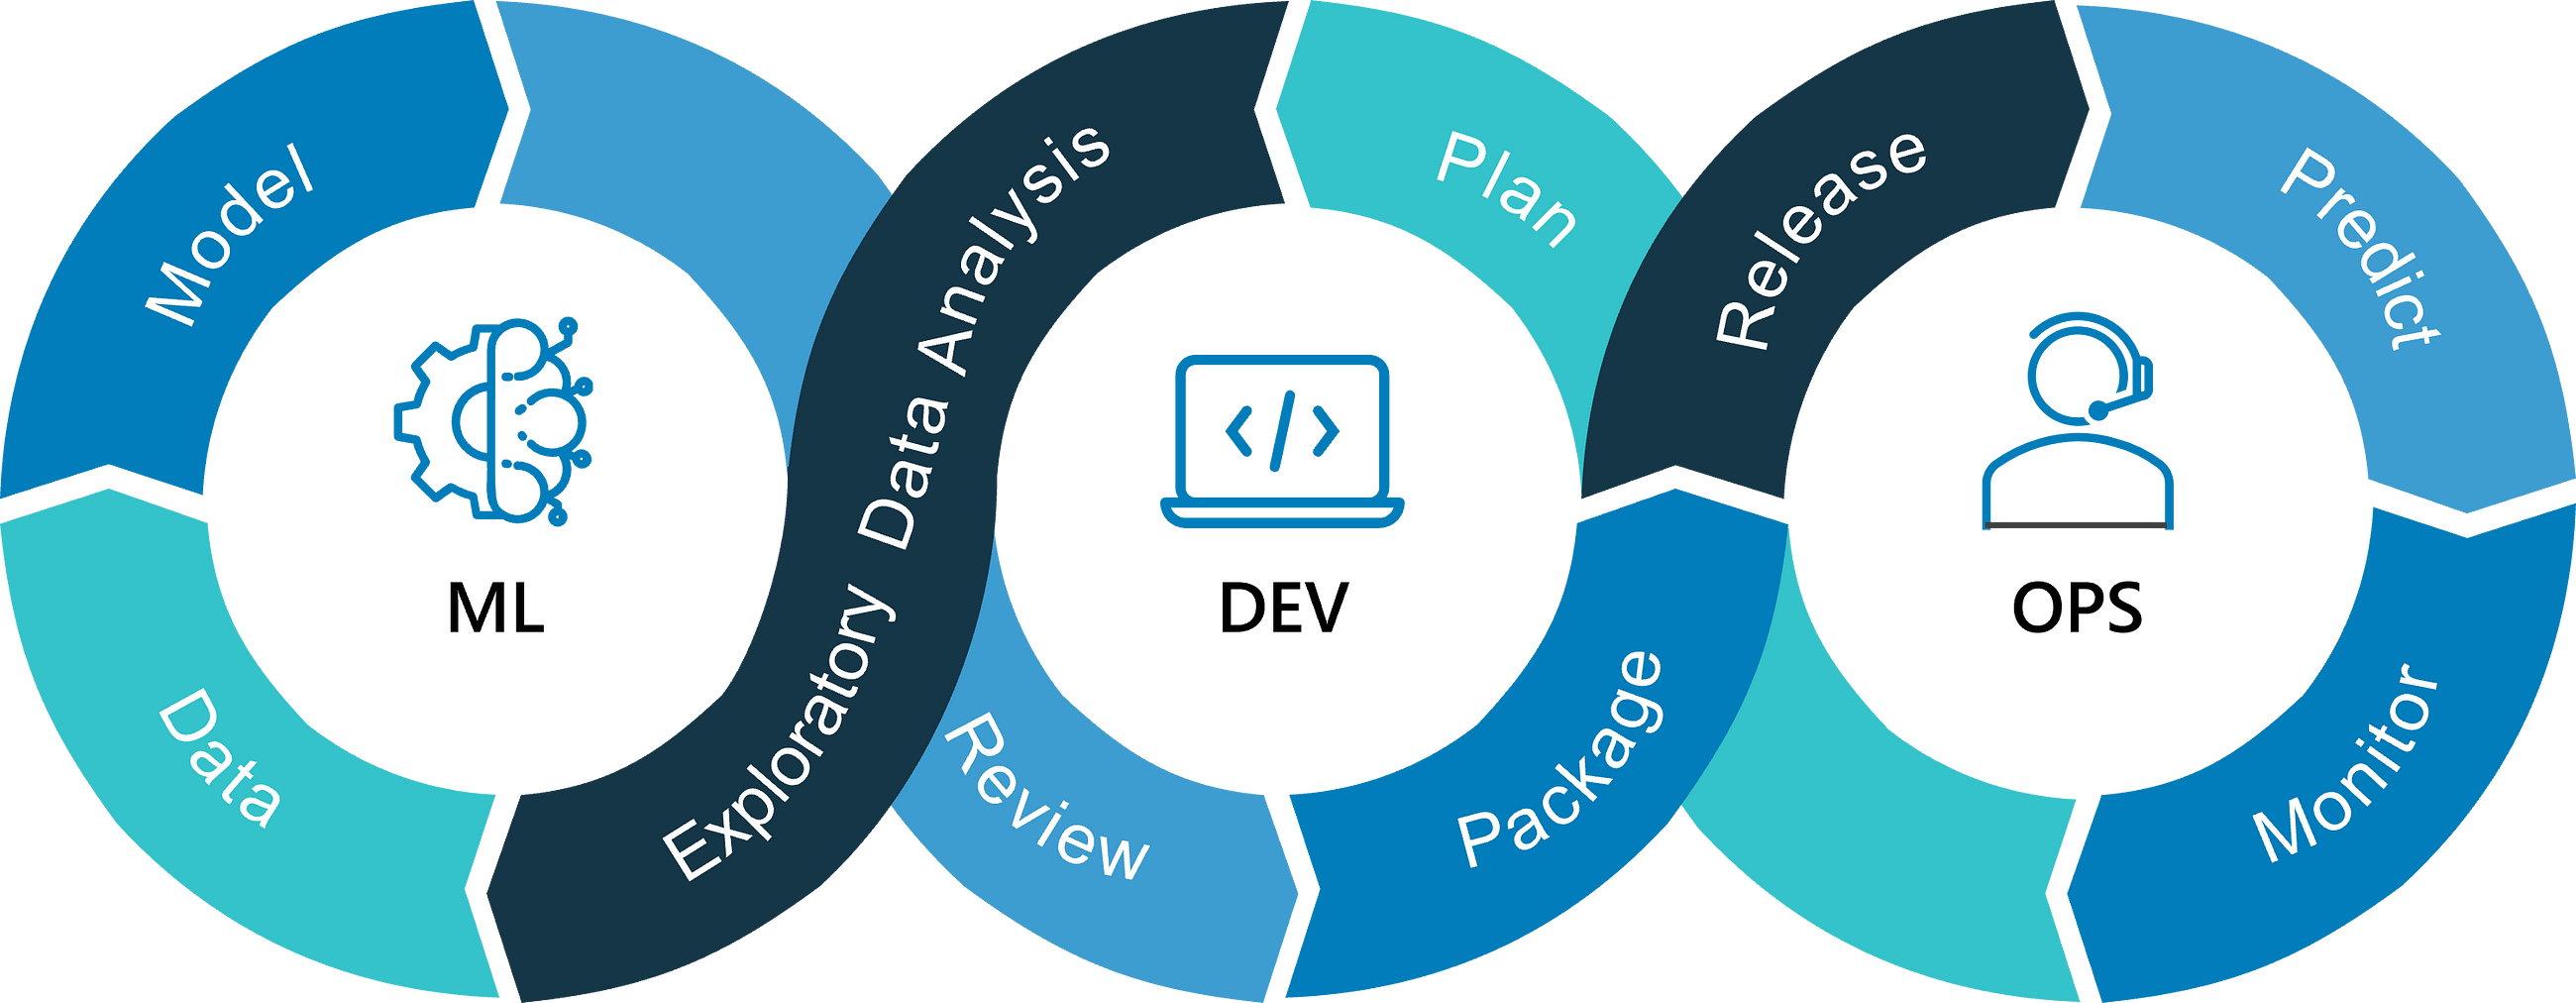
\includegraphics[width=\textwidth]{mlops-workflow.png}
    \caption{Ciclo de vida MLOps}\label{fig:mlops-workflow}
\end{figure}


Algunos de los principios clave de MLOps son:

\begin{itemize}
    \item \textbf{Automatización:} la automatización es esencial para mejorar la eficiencia del
    desarrollo de modelos y prevenir errores. Esto implica automatizar tareas como la 
    generación de datos, el despliegue de modelos, evaluación y su puesta en producción.
    \item \textbf{Colaboración y reproducibilidad:} uno de los desafíos en el Aprendizaje Automático es lograr 
    reproducir resultados de manera consistente, dada la naturaleza aleatoria de los algoritmos.
    MLOps busca, en la medida de lo posible, garantizar cierta consistencia entre los resultados
    obtenidos durante diferentes ejecuciones de un modelo para facilitar la colaboración entre
    los miembros del equipo.
    \item \textbf{Monitorización:} una vez que un modelo está en producción, es importante monitorizar
    su rendimiento para garantizar su eficacia y detectar posibles problemas. La monitorización
    permite crear alertas en caso de que el modelo no funcione correctamente y tomar medidas
    para corregirlo como por ejemplo, actualizar el modelo con nuevos datos.
    \item \textbf{Gestión de versiones:} controlar las versiones de los modelos y los datos es esencial
    para garantizar la reproducibilidad y la trazabilidad de los modelos. La gestión de versiones
    permite a los equipos comprender cómo ha evolucionado un modelo a lo largo del tiempo e incluso
    retroceder a versiones anteriores fuera necesario.
\end{itemize}

\subsubsection{Estudio de plataformas MLOps}
\begin{itemize}
    \item \textbf{MLflow:} MLflow es una plataforma MLOPs de código abierto para la gestión del ciclo de vida de
    los modelos. Ofrece una interfaz de usuario para el seguimiento de experimentos, la gestión de modelos 
    y la implementación de modelos en diferentes entornos. MLflow es compatible con la mayor parte de librerías de aprendizaje 
    automático, como TensorFlow o PyTorch. Uno de los puntos fuertes de MLflow es su gran comunidad, ya que es
    una de las plataformas más utilizadas en la industria. Sin embargo, no ofrece funcionalidades relacionadas con
    la gestión, evaluación o versionado de datasets ni con la exploración de los mismos. La dependencia sobre la
    plataforma varía en función de la tarea que se quiera realizar, pero en general, es una plataforma que no
    ata al usuario a su ella. La documentación se queda corta en cuestión de claridad y ejemplos, lo que puede
    dificultar la adopción de la plataforma por parte de los miembros del equipo.
    \item \textbf{ClearML:}Similar a MLflow, ClearML es una plataforma MLOps de código abierto que ofrece funcionalidades para la 
    gestión de experimentos, pero con la ventaja de incluir herramientas para la gestión, evaluación y 
    versionado de datasets. La dependencia sobre la plataforma es mínima, ya que con pocos cambios se pueden 
    lanzar experimentos y adicionalmente permite el lanzamiento de pipelines, gestión de alertas, orquestación de modelos 
    y generación de puntos de acceso para modelos ya desplegados. Aunque es compatible con muchas bibliotecas populares su comunidad 
    es más limitada, lo que puede dificultar a la hora de encontrar soluciones a ciertas problemáticas.
    La documentación es clara y ofrece ejemplos en formato tanto en formato de blog como de video facilitando la 
    comprensión. Sin embargo, carece de un sólido sistema de autenticación por defecto, lo que requiere una
    implementación adicional para proteger correctamente la aplicación web.
    \item \textbf{Data Version Controller (DVC):} DVC y DVC Studio son dos herramientas de código abierto que
    están diseñadas para manejar grandes volúmenes de datos, modelos y experimentos. DVC
    se centra en el versionado y almacenamiento de datasets, mientras que DVC Studio se centra en la
    monitorización de experimentos, visualización de resultados y almacenamiento de modelos. Además, 
    DVC Live proporciona integraciones con un número considerable de librerías de aprendizaje automático.
    La documentación está bien estructurada aunque no es tan clara como la de ClearML, pero cuenta con una
    comunidad bastante activa. En cuanto a los aspectos negativos de DVC, la principal desventaja es que
    la curva de aprendizaje es bastante pronunciada, lo que dificulta su adopción. Otro punto en contra
    es la gran dependencia que tienen los proyectos que usan DVC, ya que se necesita de muchos archivos
    de configuración, integraciones manuales dentro del código y un dominio completo de los comandos de la
    herramienta para poder trabajar con ella.
    \item \textbf{Kedro:} TODO:
    \item \textbf{ZenML:} ZenMl es una plataforma de código abierto encargado de la orquestación de pipelines en
    proyectos de aprendizaje automático. Ofrece una experiencia de desarrollo cómoda y modular, que facilita
    la reutilización de código. Además, cuenta con integraciones para las platformas de almacenamiento
    mas populares, como AWS y Google Cloud. A diferencia de ClearMl y MLflow, este no está enfocado en la
    gestión de experimentos ya que no es una plataforma MLOps, aunque si que ofrece conexiones con esta última
    para poder redireccionar nuestros experimentos. La documentación es clara y podemos encontrar diversos repositorios 
    con ejemplos de uso o integración con otras herramientas. El problema de esta radica principalmente
    en el hecho de que al no ser una plataforma MLOps, no ofrece funcionalidades relacionadas con la gestión
    o versionado de datasets, lo que es un punto negativo para nuestro caso de uso. Otro de los problemas
    es que las plataformas que integra no comparten las mismas credenciales dentro de su capa
    gratuita, lo que dificulta en gran medida su uso. Además, dentro de la capa gratuita estas plataformas 
    funcionan de forma independiente, lo que vuelve muy complicado el trabajo con ellas. Ademas, la funcionalidad 
    de orquestación de pipelines también viene incluida en ClearML, por lo que no aporta ninguna funcionalidad 
    adicional que no este cubierta.
\end{itemize}

\subsubsection{Estudio de herramientas de visualización de datos}
\begin{itemize}
    \item \textbf{Rath:} herramienta de exploración de datasets que permite una exploración semi-automática
    de datasets. Muy fácil de utilizar, ya que cuenta con un modo copilot que te sugiere diferentes gráficos
    y estadísticas en función de los datos que estés explorando. Además, no requiere de ninguna configuración
    previa, ya que se puede utilizar directamente desde el navegador.
    \item \textbf{Apache Superset:} Apache Superset es una plataforma de visualización de datos de código abierto 
    que ofrece una amplia gama de características para explorar y visualizar datos de manera interactiva. Con una 
    interfaz intuitiva y basada en web, Superset permite a los usuarios crear paneles de control, gráficos y tablas 
    dinámicas con facilidad. Además, ofrece integraciones con diversas fuentes de datos y admite la creación de 
    paneles de control en tiempo real. Una de las fortalezas de Apache Superset es su comunidad activa y en constante 
    crecimiento, lo que garantiza un soporte sólido y una mejora continua de la plataforma. Sin embargo, la integración
    con el resto de herramientas es limitada, ya que el propio Superset requiere de un formato de datos concreto para
    poder subir los datos a la plataforma, lo que puede dificultar su integración y generar duplicidad en cuanto a los
    datos almacenados, ya que se necesitaría una copia de los datos en el formato que requiere Superset. Nuestro objetivo
    es que esta herramienta agilice el proceso de exploración de datos, por lo que no es una opción viable por el momento.
    \item \textbf{Grafana:} Grafana es una plataforma de análisis y visualización de métricas de código abierto que 
    se ha convertido en una opción popular para monitorear sistemas y aplicaciones. Con una amplia gama de complementos 
    y paneles personalizables, Grafana permite a los usuarios crear cuadros de mando y gráficos altamente personalizados 
    para visualizar datos de diferentes fuentes. Además, ofrece características avanzadas como alertas, anotaciones y 
    exploración de datos en tiempo real. Grafana es altamente modular y extensible, lo que facilita su integración con 
    diversas tecnologías y sistemas de monitoreo. El problema de Grafana es el mismo que el de Superset, ya que requiere
    de un formato de datos concreto para poder subir los datos a la plataforma, lo que puede dificultar su integración y
    generar duplicidad en cuanto a los datos almacenados. Además, de su curva de aprendizaje, que es bastante pronunciada.
\end{itemize}
\pagebreak